\documentclass[11pt, a4paper, hidelinks]{article}[08.10.2023]
    \usepackage[left=1.4cm, top=2.3cm, text={18.2cm, 25.2cm}]{geometry}
    \usepackage[utf8]{inputenc}
    \usepackage[czech]{babel}
    \usepackage[IL2]{fontenc}
    \usepackage{times}
    \usepackage{hyperref}
    \usepackage{listings}

    \usepackage[dvipsnames]{xcolor}
    \usepackage{graphicx}
    

\lstdefinestyle{CStyle}{
    language=C,
    basicstyle=\ttfamily\small,
    keywordstyle=\color{blue},
    commentstyle=\color{green},
    stringstyle=\color{red},
    identifierstyle=\color{black},
    morekeywords={uint8_t, uint16_t, uint32_t, uint64_t, size_t, ssize_t},
    morekeywords={[2]NetFlowv5, pcap_pkthdr, netflowv5, NetFlowHeader, ethhdr, iphdr, tcphdr, ProcessedFlows, sockaddr_in, sockaddr},
    keywordstyle={[2]\color{OliveGreen}},
    morekeywords={[3]MAX_FLOW_LENGTH, create_new_flow, get_flow, check_active, check_inactive, handle_flow, insert_flow, update_flow, AF_INET, SOCK_DGRAM, IPPROTO_UDP, MAX_NUMBER_FLOWS},
    keywordstyle={[3]\color{Purple}},
    showstringspaces=false,
    tabsize=4,
    frame=single,
    numbers=left,
    numberstyle=\tiny,
    numbersep=5pt,
}

\lstset{
  basicstyle=\ttfamily, % Nastaví monospace font
  frame=single,         % Ohraničení kolem kódu
  breaklines=true,      % Zalamování dlouhých řádků
}

%Konec preambule


\begin{document}

\begin{titlepage}
    \begin{center}
        
        {\Huge \textsc{Vysoké učení technické v Brně}\\[0.5em]}
        {\huge \textsc{Fakulta informačních technologií}}
        \vspace{\stretch{0.382}}
    
        {\LARGE Síťové aplikace\\[0.4em]
        NetFlow v5 exportér}
    
        \vspace{\stretch{0.618}}
        {\Large \today \hfill {Machala Roman (xmacha86)}}
    \end{center}

\end{titlepage}
%Titulni strana

\tableofcontents
\pagebreak

\section{Úvod}
    NetFlow je síťový protokol vyvinut společností CISCO, který slouží k monitorování a analýze síťového provozu.
    Umožňuje zachytávat jednotlivé pakety, které následně rozděluje do toků na základě např. zdrojové a cílové IP adresy.
    Tyto data jsou pomocí protokolu UDP z exportéru odeslána do centrálního sběrače (kolektoru), kde
    mohou být analyzována za účelem zjištění vytížení síte, anomálií nebo napříkald i bezpečnostních incidentů\cite{Cisco_2019}.

    Pro protokol NetFlow existuje mnoho verzí, nicméně tato práce se 
    zabývá pouze verzí v5, což je jedna z nejpoužívanějších verzí vůbec, dostupná na drtivé většině
    zařízení různých výrobců. Tato verze byla navržena pro sběr informací síťového
    provozu pouze na bázi IPv4. Pro podporu IPv6 je nutno vuyžívat vyšších verzí, jako je například NetFlow v9\cite{ManageEngine}.

\subsection{IP Tok}\label{tok}
    Jak již bylo zmíněno výše, protokol NetFlow pracuje s jednotlivými paketami, které rozděluje do \textbf{toků}.
    Každý takový tok je určen unikátní kombinací následujících informací:
    \begin{itemize}
        \item{\textbf{Zdrojová IP adresa}}
        \item{\textbf{Cílová IP adresa}}
        \item{\textbf{Zdrojový PORT}}
        \item{\textbf{Cílový PORT}}
        \item{Typ služby (ToS)}
        \item{\textbf{Protokol 3 vrstvy}}
        \item{Rozhranní}
    \end{itemize}

    Všechny toky jsou pouze jednosměrné, proto například prohozením adres odesílatele a příjemce nevznikne
    nový tok, jak je demonstrováno na obrázku \ref{priklad1}. V rámci implementace popsané v této práci jsou ovšem za unikátní identifikátory uvažovány
    pouze \textbf{tučně} vyznačené informace. Je tak uvažováno z důvodů stanovení požadavků dle zadání nebo pozdějších upřesnění v rámci diskuzního fóra pro řešení projektu. Více info o rozdílech a limitacích v sekci \ref{limitace}.
    \vspace{2cm}

    \begin{figure}[h!]
        \begin{minipage}[t]{0.45\textwidth}
            \subsection*{Tok 1:}
            \begin{tabbing}
                \hspace*{4cm}\=\hspace*{4cm}\= \kill
                Zdrojová IP: \> 192.168.1.1 \\
                Cílová IP: \> 10.0.0.1 \\
                Zdrojový port: \> 12345 \\
                Cílový port: \> 80 \\
                Protokol: \> TCP \\
            \end{tabbing}
        \end{minipage}
            \hfill
        \begin{minipage}[t]{0.45\textwidth}
            \subsection*{Tok 2:}
            \begin{tabbing}
                \hspace*{4cm}\=\hspace*{4cm}\= \kill
                Zdrojová IP: \> 10.0.0.1 \\
                Cílová IP: \> 192.168.1.1 \\
                Zdrojový port: \> 80 \\
                Cílový port: \> 12345 \\
                Protokol: \> TCP \\
            \end{tabbing}
        \end{minipage}
        \caption{Příklad 2 různých toků}
        \label{priklad1}
    \end{figure}

    Z obrázku \ref{priklad1} může být taky patrné, že protokol nebere ohled na obsah jednotlivých paket, co se týče rozdělení paket do toků.
    V rámci protokolu NetFlow v5 se s obsahem paket nijak nemanipuluje, uchovávají se ovšem další informace, které jsou vhodné pro 
    statistické vyobrazení a monitorování síťového provozu.
    
    \subsection{Struktura toků/NetFlow v5 datagram}\label{Datagram}
    Kromě klíčových informací sloužících k rozdělení jednotlivých paket do toků se ukládají i jiné informace o každém toku.
    Výčet těchto informací je vyobrazen jako struktura v jazyce C na obrázku \ref{netflowstruct}. V tomto formátu jsou jednotlivé toky
    pomocí UDP protokolu odeslány na kolektor. 
    
    Jelikož je používán protokol UDP pro export datagramů, je možné, že některé datagramy mohou být 
    ztraceny. Z tohoto důvodu novější verze tohoto protokolu, přesněji verze 5, 7 a 8 obsahuje hlavička, dále popsána na obrázku \ref{netflowhdr}, kontrolní číslo toku (\textbf{flow control number}), které je 
    rovno kontrolnímu číslu předešlého toku + počet toků v předešlém datagramu. Při přijetí nového datagramu tak kolektor může zkontrolovat, zda došlo 
    ke ztrátě toků\cite{Cisco_datagram}\cite{IBM_header}.

    \begin{figure}[h!]
        \centering
        \begin{lstlisting}[style=CStyle]
            typedef struct NetFlowv5 {
                uint32_t srcaddr;       /* Source IP address */
                uint32_t dstaddr;       /* Destination IP address */
                uint32_t nexthop;       /* IP address of next hop router */
                uint16_t input;         /* SNMP index of input interface */
                uint16_t output;        /* SNMP index of output interface */
                uint32_t dPkts;         /* Packets in the flow */
                uint32_t dOctets;       /* Total number of Layer 3 bytes */
                uint32_t first;         /* SysUptime at start of flow */
                uint32_t last;          /* SysUptime at the time the last packet */
                uint16_t srcport;       /* TCP/UDP source port number */
                uint16_t dstport;       /* TCP/UDP destination port number */
                uint8_t pad1;           /* Unused (zero) bytes */
                uint8_t tcp_flags;      /* Cumulative OR of TCP flags */
                uint8_t prot;           /* IP protocol type (for example, TCP = 6) */
                uint8_t tos;            /* IP type of service (ToS) */
                uint16_t src_as;        /* Autonomous system number of the source */
                uint16_t dst_as;        /* Autonomous system number of the dest */
                uint8_t src_mask;       /* Source address prefix mask bits */
                uint8_t dst_mask;       /* Destination address prefix mask bits */
                uint16_t pad2;          /* Unused (zero) bytes */
            } netflowv5;
        \end{lstlisting}
        \caption{NetFlow v5 tělo datagramu}
        \label{netflowstruct}
    \end{figure}

    \begin{figure}[h!]
        \centering
        \begin{lstlisting}[style=CStyle]
            typedef struct NetFlowHeader {
                uint16_t version;            /* NetFlow export format version num */
                uint16_t count;              /* Number of exported flows */
                uint32_t sysUptime;          /* Current time in ms since start */
                uint32_t unix_secs;          /* Current count of seconds since CUT */
                uint32_t unix_nsecs;         /* Residual nanoseconds since CUT */
                uint32_t flow_sequence;      /* Sequence cnt of total flows seen */
                uint8_t engine_type;         /* Type of flow-switching engine */
                uint8_t engine_id;           /* Slot num of flow-switching engine */
                uint16_t sampling_interval;  /* Sampling mode + interval (2b - 14b) */
            } NetFlowHeader;
        \end{lstlisting}
        \caption{NetFlow v5 hlavička datagramu}
        \label{netflowhdr}
    \end{figure}

    \subsection{Expirace toků}\label{timeout}
    Jednotlivé toky je nutno v určitém okamžiku uzavřít a připravit je pro odeslání na kolektor.  V rámci protokolu NetFlowv5 se řeší 2 typy timeoutů, kdy je tok považován za expirovaný/uzavřený.

    \subsubsection{Aktivní timeout}
    Aktivní timeout stanovuje dobu od první přijaté pakety, po které je tok uzavřen, nehledě na tom, zdali přicházejí další pakety. Jednoduchým příkladem může být komunikace mezi bodem \textbf{A} a \textbf{B}, která trvá 5 minut, tedy (300 sekund). Pokud bude aktivní timeout nastaven na dobu 60 sekund, z této komunikace nám vznikne celkem 5 toků, které budou identické co se týče položek určujících tok, sekce \ref{tok}, ale mohou být různé v počtu paket a celkového počtu bytů v rámci jednotlivých toků.

    \subsubsection{Neaktivní timeout}
    Neaktivní timeout stanovuje dobu od poslední přijaté pakety, po kterou pokud nedojde další paketa patřící do onoho toku, je tok uzavřen. Příkladem pro tok expirovaný/uzavřený na základě neaktivního timeoutu je komunikace mezi bodem \textbf{A} a \textbf{B}, která obsahuje 2 pakety, kdy paketa \textbf{P1} je zachycena v čase \textbf{T1} a paketa \textbf{P2} je zachycena v čase \textbf{T1 + 30s}. Pokud je neaktivní timeout nastaven na 20 sekund, bude v době \textbf{T1 + 20s} tok obsahující pouze paketu \textbf{P1} uzavřen. Pro následující paketu \textbf{P2} v čase \textbf{T1 + 30s} bude vytvořen nový tok, obsahující pouze paketu \textbf{P2}.
    
    \subsection{Rozdíly v implementaci}\label{limitace}
    V této sekci jsou popsány limitace procesu návrhu a implementace exportéru pro protokol NetFlow v5. 
    
    Implementovaný exportér pracuje pouze s informacemi zjistitelnými analýzou zachycených paket z poskytnutého PCAP souboru.
    Mezi nezjistitelné položky tak patří:

    \begin{itemize}
        \item{Adresa routeru dalšího skoku}
        \item{SNMP indexy vstupního a výstupního zařízení}
        \item{Čísla autonomních sýstémů zdrojové a cílové sítě}
        \item{Počet bitů v maskovacím prefixu zdrojové a cílové adresy}
        \item{Typ a ID zařízení zpracovávající toky}
        \item{Sampling mód a interval}
    \end{itemize}

    Takto nezjistitelné informace jsou potom nahrazeny 0, což je standardní postup při analýze paket z PCAP souboru.

    Dalším omezením jsou časové značky jednotlivých toků a paket. NetFlowv5 uchovává informace jako je třeba čas zachycení pakety od spuštění exportéru.


    \begin{equation}
        x = T1 - T0
    \end{equation}
    Kde $x$ představuje čas zachycení pakety od spuštění systému, $T1$ skutečný čas zachycení pakety a $T0$ skutečný čas spuštění exportéru.
    Jelikož ale pakety byly zachyceny před spuštěním exportéru, musí platit, že:

    \begin{equation}
        T1 < T0
    \end{equation}
    a z toho důvodu jsou jednotlivé časové značky záporné. Drtivá většina kolektorů ovšem s tímto faktem počítá a záporné hodnoty jsou interpretovány bez problémů.

    TCP flagy RST a FIN nejsou brány v potaz a neukončují tak tok, jak je tomu zvykem u některých NetFlow exportérů.

    Z důvodu kontroly expirace toků až v momentě, kdy jsou vkládány nové informace do toku, popsáno v sekci \ref{kontrola}, může nastat situace, že do toku již nemusí přijít nové informace a tok tak bude exportován až v případě kompletního zpracování souboru, tedy pořadí exportovaných toků nemusí odpovídat jejich skutečnému pořadí expirace\footnote{Snažil jsem se tomuto více věnovat zkoumáním softflowd a nfcapd nástrojů a ve výsledků se nic nestane, jen nesedí jejich pořadí.}.
    
    \section{Návrh a implementace}
    Samotná aplikace je rozdělena do několika větších celků, kde každý celek zajišťuje určitou část aplikace. Jednotlivé celky jsou implementovány v 
    samostatných \texttt{.c} a \texttt{.h} souborech. Jednotlivé celky dohromady potom tvoří výslednou aplikaci pracující jako exportér
    NetFlow v5 toků.

    \subsection{Zpracování argumentů}
    Tento celek se stará o zpracování argumentů příkazové řádky, poskytnuté uživatelem, převodem těchto argumentů
    do jejich očekávané podoby (pokud je to potřeba), nebo ke kontrole jejich správnosti.

    \begin{table}[ht]
        \centering
        \begin{tabular}{|l|l|l|}
        \hline
        \textbf{Parametr}         & \textbf{Popis}                                                  & \textbf{Povinný}  \\ \hline
        \texttt{hostname:port}    & IP adresa a port kolektoru                                      & Ano              \\ \hline
        \texttt{pcap\_soubor}     & PCAP soubor obsahující pakety pro analýzu                       & Ano              \\ \hline
        \texttt{-a | --active}         & Aktivní timeout v sekundách                                     & Ne               \\ \hline
        \texttt{-i | --inactive}         & Neaktivní timeout v sekundách                                   & Ne               \\ \hline
        \texttt{-d | --debug}               & Povolit ladicí výstup                                           & Ne               \\ \hline
        \end{tabular}
        \caption{Parametry aplikace}
        \label{parametry}
    \end{table}
        
    V tabulce \ref{parametry} je možno vidět, jaké parametry aplikace podporuje. Na jejich pořadí nezáleží, ovšem povinné parametry
    musejí být vždy přítomny. Pokud nejsou stanoveny parametry \textbf{-a} a \textbf{-i}, tedy aktivní a neaktivní timeout, pracuje se s 
    defaultní hodnotou 60 sekund pro oba timeouty.

    \subsection{Zpracování paket ze souboru PCAP}
    Pro zpracování jednotlivých paket a jejich manipulace s nimi je prováděna výhradně za pomocí knihovny PCAP. Mezi nejdůležitější funkce používáné pro tento účel jsou \texttt{pcap\_open\_offline()} a \texttt{pcap\_loop()}, které umožňují otevřít samotný soubor a načítat postupně pakety\cite{Pcap_open_offline}\cite{Pcap_loop}.

    Jednotlivé pakety josu pak načteny v následujícím formátu:
    \vspace{1cm}

    \begin{table}[ht]
        \centering
         \begin{tabular}{|c|c|c|c|c|}
            \hline
                \color{red}PCAP hlavička  &  \color{blue}Ethernetová hlavička & \color{blue}IP hlavička & \color{blue}TCP hlavička & \color{blue}Data \\
            \hline
        \end{tabular}
        \caption{Zachycená paketa}
        \label{paketa}
    \end{table}

    \vspace{1cm}

    V tabulce \ref{paketa} je paketa barevně odlišena na 2 části, se kterými se dá dále manipulovat.
    \pagebreak

     \begin{figure}[h]
        \centering
        \begin{lstlisting}[style=CStyle]
            struct pcap_pkthdr *pkthdr;     /* PCAP header */
            uint8_t *packet;                /* Packet */

            /* Get ethernet header */
            struct ethhdr *ether_header = (struct ethhdr *)packet;

            /* Get IP header */
            struct iphdr *ip_header = (struct iphdr *)(packet + 
                    sizeof(struct ethhdr));

            /* Get TCP header */
            struct tcphdr *tcp_header = (struct tcphdr *)(packet + 
                    sizeof(struct ethhdr) + (ip_header->ihl * 4));
            
        \end{lstlisting}
        \caption{Práce s paketami}
        \label{paketa_c}
    \end{figure}

    Na obrázku \ref{paketa_c} je vyobrazena následná práce s jednotlivými částmi zachycené pakety a jak se dostat k jedjnotlivým položkám popsaných v tabulce \ref{paketa}. Samotná data nás již nijak nezajímají, jelikož všechny potřebné informace se nachází v jendotlivých hlavičkách\cite{Pcap_general}.

    \subsection{Tvorba toků}
    Obrázek \ref{paketa_c} nám popisuje jak dostaneme jednotlivé hlavičky ze zachycené pakety. Samotné informace pro tvorbu toku, popsáno v sekci \ref{tok}, jsme již schopni získat poměrně snadno.

    Pro každou paketu je vytvořena struktura popsána na obrázku \ref{netflowstruct} a jsou vyplněny všechny možné informace, které jsou dostupné z jednotlivých hlaviček paket. Následně je tok zkontrolován, zdali již neexistuje a na základě toho, je buďto aktualizován již existující tok nebo uložen nový.

    \subsection{Struktura pro ukládání toků}
    Jakožto struktura uchovávající jednotlivé záznamy o všech tocích je zvolena mírně upravená hashovací tabulka. Na základě potřebných informací tvořící unikátní kombinaci toku, sekce \ref{tok}, je vypočítán hash udávající index umístění toku v tabulce. Postup výpočtu hashe je možno vidět na obrázku \ref{hash}.

     \begin{figure}[h!]
        \centering
        \begin{lstlisting}[style=CStyle]
            int hash_function(netflowv5 *flow){
                uint64_t hash = flow->srcaddr;
                hash ^= flow->dstaddr;
                hash ^= (flow->srcport << 16);
                hash ^= (flow->dstport << 16);
                hash ^= (flow->prot << 16);
            
                return hash % MAX_FLOW_LENGTH;
            }
        \end{lstlisting}
        \caption{Výpočet hashe}
        \label{hash}
    \end{figure}

    \subsection{Kontrola expirace toků}\label{kontrola}
    Před vložením jednotlivých toků do tabulky je třeba zkontrolovat zdali neexistuje již takový tok v tabulce a pokud ano, jestli může být tok aktualizován, aby neporušil některý z timeoutů, popsaných v sekci \ref{timeout}.

    Logika vkládání a kontroly je popsána v pseudokódu na obrázku \ref{pseudo}.

     \begin{figure}[ht]
        \centering
        \begin{lstlisting}[style=CStyle]

            /* Creates new flow based on provided packet */
            flow = create_new_flow()

            /* If same flow already exists, finds it */
            orig_flow = get_flow(flow)

            /* if it exists */
            if orig_flow: 
                /**
                * Checks wheter by updating original flow either active or inactive
                * timeout is exceeded
                */
                if check_active(orig_flow, flow) or check_inactive(orig_flow, flow):
                    /* Closes flow and removes it from table */
                    handle_flow(orig_flow)
                    /* Inserts new flow into table */
                    insert_flow(flow)
                else:
                    /* Updates flow if no timeoutes are exceeded */
                    update_flow(orig_flow, flow)
            else:
                /* if no flow is found then insert as a new flow */
                insert_flow(flow)

            
        \end{lstlisting}
        \caption{Vkládání a kontrola expirace}
        \label{pseudo}
    \end{figure}

    \pagebreak

    Základní princip spočívá v tom, že při načtení pakety je vytvořen nový tok, následně se vyhledá v tabulce, zdali již takový tok neexistuje. Pokud ne, je nový tok vložen do tabulky. Pokud ano, zkontroluje se, pokud aktualizací již existujícího toku dojde k překročení nějakého z timeoutů, je původní tok uzavřen a uchován ve struktuře pro export toků, více v sekci \ref{export}, a nově vytvořený tok je vložen do tabulky. Pokud k překročení timeoutu nedojde, je původní tok aktualizován nově vytvořeným.
    
    \subsection{Export toků}\label{export}
        Všechny uzavřené toky jsou uchovávány ve struktuře popsané na obrázku \ref{set}. Úkolem této struktury je uchovávat jednotlivé toky, považované za uzavřené na jednom místě, dokud nedojde k jejich exportu na kolektor. Aby byl počet exportovaných toků využit na maximum, dochází k jejich exportu, pokud je jejich počet roven 30, nebo pokud se zpracovaly všechny pakety ze souboru. 

     \begin{figure}[h!]
        \centering
        \begin{lstlisting}[style=CStyle]
            typedef struct ProcessedFlows{
                int count;                              /* Current num of flows */
                int total_count;                        /* Num of flows */
                netflowv5 *flows[MAX_NUMBER_FLOWS];     /* Flows */
            }ProcessedFlows;
            
        \end{lstlisting}
        \caption{Struktura pro uzavřené toky}
        \label{set}
    \end{figure}

    Položka \textbf{count} uchovává počet aktuálně uzavřených toků a při její hodnotě rovno 30 dojde k exportu. \textbf{Count} je pak resetován a inkrementován s dalším přibývajícím tokem. Položka \textbf{total\_count} potom slouží k uchování celkového počtu všech toků, pro naplnění kontrolního počtu toků v hlavičce NetFlowv5 protokolu, viz. obrázek \ref{netflowhdr}

    Samotnou logiku pro vytvoření datagramu pro export toků lze pak vidět na obrázku \ref{export_udp}.
         \begin{figure}[ht]
        \centering
        \begin{lstlisting}[style=CStyle]
            NetFlowHeader header;
            /* Fill header info */
            ...
            /* Create socket and check for succes */
            int sock = socket(AF_INET, SOCK_DGRAM, IPPROTO_UDP);
            ...
            /* Fill colector address */
            struct sockaddr_in collector_addr;
            ...
            /* Calculate UDP size and allocate memory */
            size_t packet_size = sizeof(header) + 
                    sizeof(struct NetFlowv5) * set.count;
            uint8_t *buffer = malloc(packet_size);

            /* Copy header data to buffer */
            memcpy(buffer, &header, sizeof(header));
            /* Copy all flows into buffer */
            for(int i = 0; i < set.count; i++){
                convert_flow_to_network_order(set.flows[i]);
                memcpy(buffer + sizeof(header) + 
                        (i * sizeof(struct NetFlowv5)), set.flows[i], 
                            sizeof(struct NetFlowv5));
            }
            /* Send datagram to collector */
            ssize_t sent_bytes = sendto(sock, buffer, packet_size, 0, 
                    (struct sockaddr*)&collector_addr, 
                    sizeof(struct sockaddr_in));
            ...
        \end{lstlisting}
        \caption{Tvorba datagramu}
        \label{export_udp}
    \end{figure}

    \pagebreak
    
    \section{Testování aplikace}\label{test_zac}
    Pro zajištění správného chodu aplikace, byla jednak v průběhu implementace řádně zkoumána řadou nástrojů, ale taktéž důkladně testována. Většina těchto nástrojů je považována za referenční, proto je testování uzpůsobeno porovnávání výsledků implementovaného exportéru a referečních nástrojů. Více o těchto nástrojích v sekci \ref{refer_nastroje}. Testy jsou plně automatizované a jsou dostupné ve složce \texttt{/tests}. Samotné testování je pak možno spustit následovně:

    \begin{center}
        sudo ./tests.sh
    \end{center}
    kde je potřeba se nacházet ve složce \texttt{/tests}.
    \subsection{Návrh testů}\label{test_navrh}
    Samotné testy jsou rozvrženy do několika skupin, kde každá skupina se snaží otestovat jinou část programu. 

    \begin{itemize}
        \item{Nejjednoduší testy se zabývají zpracováním 3-5 paket, kde všechny pakety patří do stejného toku. Cílem je tak ověřít schopnost programu zpracovat primitivní možství paket a samotnou schopnost vytvoření toku a následné agregace příslušných paket do oneho toku. Jsou zpracovávány zachycené komunikace obsahující pouze TCP protokol.} 
        \item{Pokročilější testy jsou uzpůsobeny pro kontrolu schopnosti programu zpracovávat větší množství paket, cca 150, patřících do různých toků. Důklad je tedy kladen na správnou tvorbu toků, agregaci nových paket do toků a správnou manipulaci s pamětí.}
        \item{Náročnější testy potom kombinují vělké množství paket a různé protokoly. Cílem je opět správně zapracovat pakety do příslušných toků, správná manipulace s pamětí a zpracování pouze TCP paket.}
        \item{Samostatnou skupinu potom tvoří testy pro kontrolu správné implentace jednotlivých timeoutů, viz sekce \ref{timeout}. V těchto testech je primární zaměření na korektní tvorbu toků v závislosti na jednotlivých timeoutech. Pracuje se s menším množstvím paket, aby bylo zřetelné množství jednotlivých toků, nicméně je předpokládáno, že je možno zpracovávat libovolné množství paket\footnote{Tyto testy jsou jediné, jež nejsou automatizované.}.}
    \end{itemize}
  
    \subsection{Referenční programy a jejich použití}\label{refer_nastroje}
    V této sekci jsou popsány jednotlivé nástroje použity pro účely ladění programu, testování anebo pro zkoumání jejich chování. U jednotlivých nástrojů je taky popsáno, jakým způsobem jsou nástroje spouštěny a k čmeu byly přesně použity.
    \subsubsection{Wireshark}
    Program Wireshark je použit především pro zachycení komunikace pro samotné testy a pro zkoumání detailů implementace nástroje Softflowd. Komunikace byla zachycena na počítači s kabelovým internetovým připojením na rozhraní \texttt{eth0}.
    \subsubsection{Softflowd}
    Nástroj softflowd slouží jako referenční exportér. Byl využit jednak pro zkoumání detailů implementace, ale i pro generování referenčních výsledků, kterých by měl implementovaný exportér dosáhnout.

    Nástroj byl spouštěn následovně:
    \begin{center}
        softflowd -r FILE -n localhost:1010 -v 5 -d\footnote{Export paketů ze souboru FILE na kolektor na adrese localhost:1010, verze NetFlowv5}
    \end{center}

    \subsubsection{Tcpdump}
    Tento nástroj byl především použit pro filtraci paket pro jednotlivé testy. Některé ze zachycených komunikací pro účely testování obsahují protokoly i jiné, než TCP. Z tohoto důvodu jsou testovací pakety před zpracováním nástrojem softflowd přefiltrovány, aby obsahovaly pouze pakety s protokolem TCP. Tato filtrace je ovšem použita pouze před použitím referenčního nástroje, který neumožňuje, například přepínačem, zpracovávat pouze určité druhy protokolů. Implementovaný exportér zpracovává pouze TCP, není tedy nutná filtrace před jeho použitím.
    Nástroj byl spouštěn následovně:

    \begin{center}
        tcpdump -r FILE -w FILTERED\_FILE -p tcp\footnote{Filtrace tcp paket ze souboru FILE, zápis do souboru FILTERED\_FILE}
    \end{center}

    \subsubsection{Nfcapd}\label{collector}
    Tento nástroj byl použit jako kolektor pro jednak referenční exportér, ale i pro implementovaný. Jeho úkolem bylo zachycení exportovaných toků a vyobrazení jednotlivých statistik, jejichž shoda pak znamenala úspěch daného testu.
    Nástroj byl spouštěn následovně:

    \begin{center}
        nfcapd -l OUTPUT\_DIR -p 1010\footnote{Výstup nástroje uložen do složky OUTPUT\_DIR, poslouchá na portu 1010}
    \end{center}

    \subsubsection{Nfdump}
    Nfdump slouží pro vyobrazení jednotlivých statisktik, jež jsou výstupem kolektoru. 
    Jedná se tak o nástroj zobrazující statistiky zpracovaných exportovaných toků. Tyto statistiky jsou následně klíčové pro ověření správnosti implementovaného exportéru vůči referenčnímu.
    Nástroj byl spouštěn následovně:
    \begin{center}
        nfdump -r FILE\footnote{Zobrazí statistiky daného souboru}
    \end{center}

    \subsubsection{Valgrind}
    Nástroj valgrind byl využit pro kontrolu práce s pamětí, její alokace a především její správné uvolnění. Každý test kromě kontroly požadovaných statistik kontroluje i správu paměti, která je jednou z mnoha podmínek pro splnění daného testu.
    \subsection{Podmínky testování}\label{test_podm}
    Samotné testování funguje na tom principu, že je spuštěn kolektor a jsou na něj odeslány toky z referenčního a implementovaného exportéru. Klíčové vlastnosti, které jsou kontrolovány jsou následující:
    \begin{itemize}
        \item{Správná manipulace s pamětí}
        \item{Celkový počet toků}
        \item{Celkový počet bytů}
        \item{Celkový počet paket}
        \item{Celkový počet zpracovaných toků}
        \item{Počet přeskočených bloků}
        \item{Přečteno bytů}
        \item{Časová okna toků}
    \end{itemize}

    Položky jako průměrný počet paket za sekundu atd. jsou taktéž kontrolovány, ale v případě neshody jsou pouze vypsaný, nejsou brány jako důvod k označení testu za selhaný, protože tyto informace vyžadují vysokou časovou přesnost a jsou závislé na celkové době zpracování toků, což může být ovlivněno specifickou implementací. Příklad, jak vypadají kontrolované položky je na obrázku \ref{test_pr}.

    \begin{figure}[ht]
        \centering
        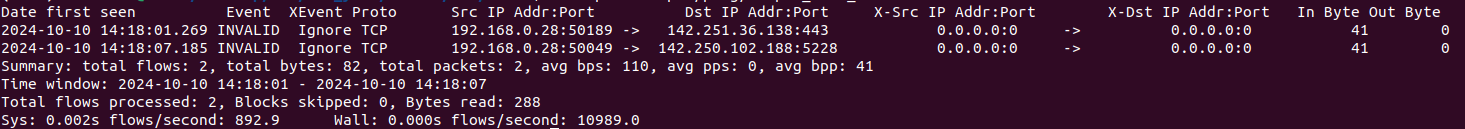
\includegraphics[width=1\linewidth]{pictures/test_pr.png}
        \caption{Příklad výstupu}
        \label{test_pr}
    \end{figure}
    
    \subsection{Provedení testování}
    Samotné testování proběhlo v pořádku. Pro jednotlivé testy zaměřující se na klíčové vlastnosti programu, viz. sekce  \ref{test_navrh}, jsou všechny testy průchozí v souladu s podmínkami v sekci \ref{test_podm}. Tyto testy jsou automatizované a  je tak možno si je snadno zreplikovat, viz úvod sekce \ref{test_zac}. Testování timeoutů probíhalo ručně, jelikož nebyla možnost specificky nastavit tyto hodnoty u referenčního exportéru, tudíž se testy nedaly zautomatizovat. Následující část popisuje toto testování a zobrazuje jejich vstupní data a jejich výsledky\footnote{Kolektor v následujících testech byl spouštěn v souladu s popisem v sekci \ref{collector}}.
        \pagebreak
    \subsubsection{Testování aktivního timeoutu}

    \begin{center}
        ../p2nprobe localhost:1010 timeouts/z\_timeout\_test\_0.pcap -a 1
    \end{center}
    \vspace{1cm}
    \begin{figure}[ht]
        \centering
        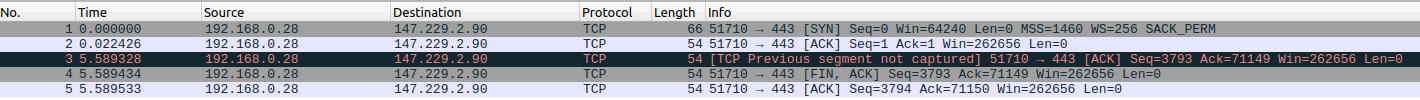
\includegraphics[width=1\linewidth]{pictures/test_1_data.png}
        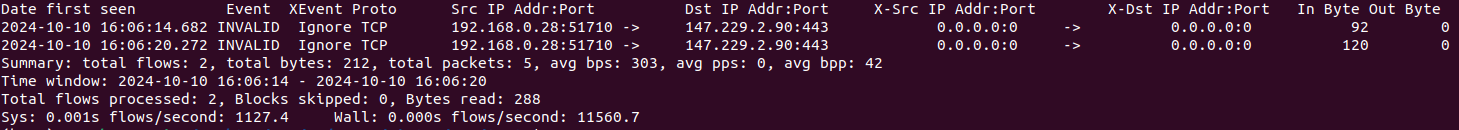
\includegraphics[width=1\linewidth]{pictures/test_1_res.png}
        \caption{Test 1}
    \end{figure}

    \begin{center}
        ../p2nprobe localhost:1010 timeouts/z\_timeout\_test\_0.pcap -a 5
    \end{center}
    \vspace{1cm}
    \begin{figure}[ht]
        \centering
        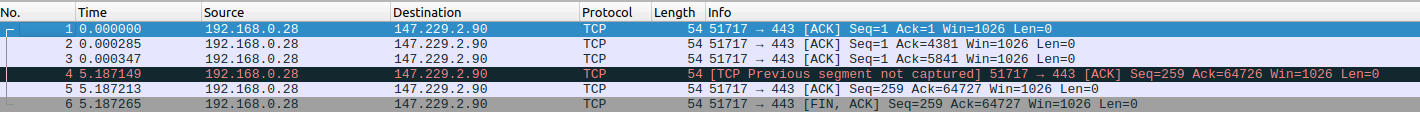
\includegraphics[width=1\linewidth]{pictures/test_2_data.png}
        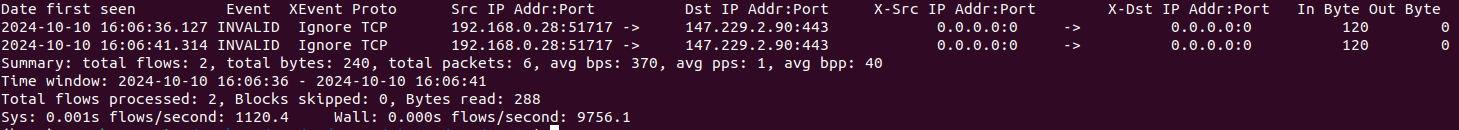
\includegraphics[width=1\linewidth]{pictures/test_2_res.png}
        \caption{Test 2}
    \end{figure}

    \begin{center}
        ../p2nprobe localhost:1010 timeouts/z\_timeout\_test\_0.pcap -a 4
    \end{center}
    \vspace{1cm}
    \begin{figure}[ht]
        \centering
        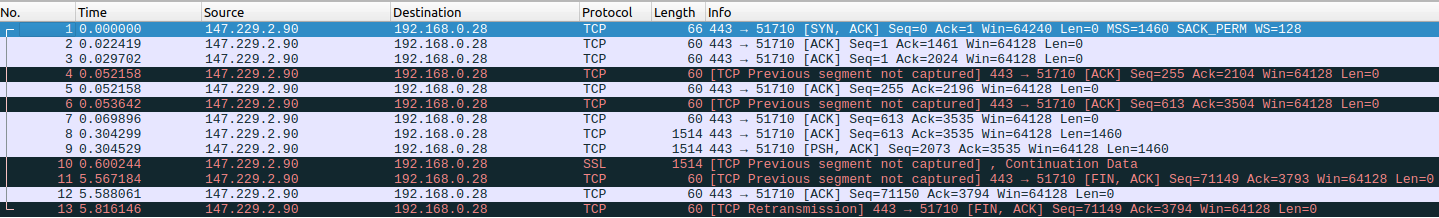
\includegraphics[width=1\linewidth]{pictures/test_3_data.png}
        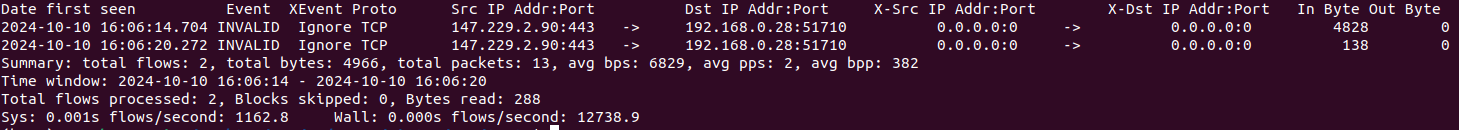
\includegraphics[width=1\linewidth]{pictures/test_3_res.png}
        \caption{Test 3}
    \end{figure}

    \pagebreak
    \subsubsection{Testování inaktivního timeoutu}
    \begin{center}
        ../p2nprobe localhost:1010 timeouts/z\_timeout\_test\_0.pcap -i 4
    \end{center}
    \begin{figure}[ht]
        \centering
        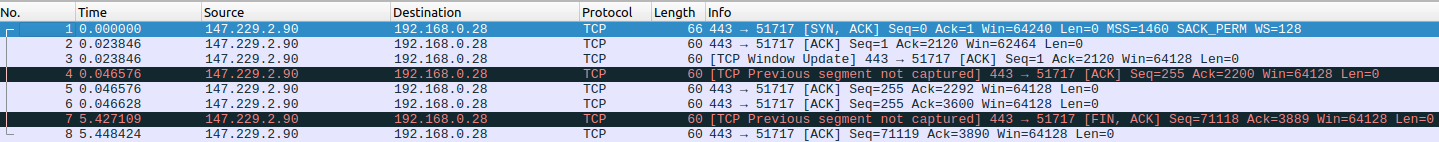
\includegraphics[width=1\linewidth]{pictures/test_4_data.png}
        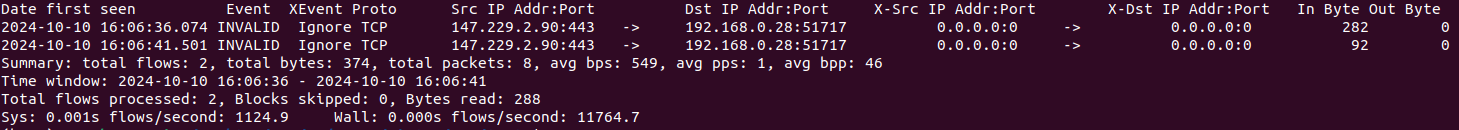
\includegraphics[width=1\linewidth]{pictures/test_4_res.png}
        \caption{Test 4}
    \end{figure}

    \begin{center}
        ../p2nprobe localhost:1010 timeouts/z\_timeout\_test\_0.pcap -i 5
    \end{center}
    \begin{figure}[ht]
        \centering
        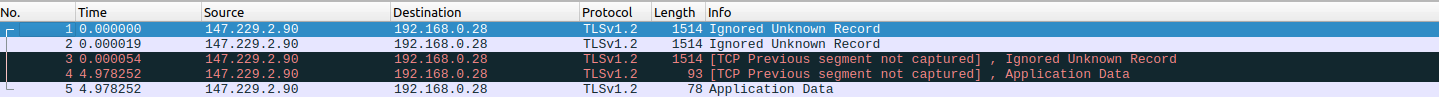
\includegraphics[width=1\linewidth]{pictures/test_5_data.png}
        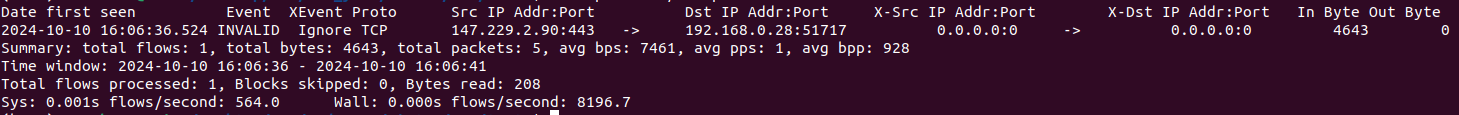
\includegraphics[width=1\linewidth]{pictures/test_5_res.png}
        \caption{Test 5}
    \end{figure}

    \begin{center}
        ../p2nprobe localhost:1010 timeouts/z\_timeout\_test\_0.pcap -i 2
    \end{center}
    \begin{figure}[ht]
        \centering
        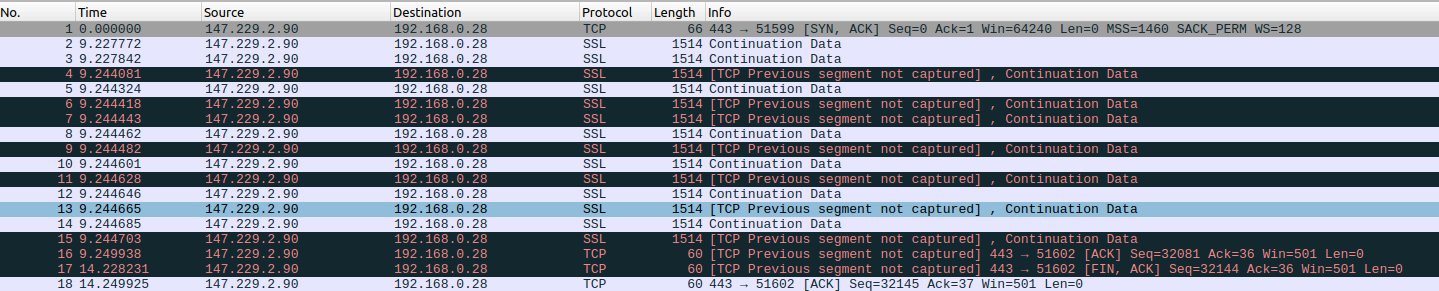
\includegraphics[width=1\linewidth]{pictures/test_6_data.png}
        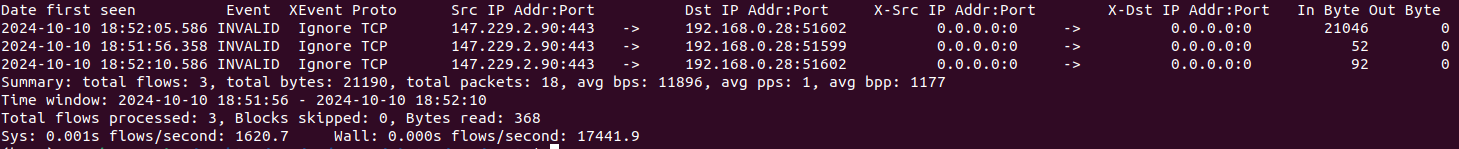
\includegraphics[width=1\linewidth]{pictures/test_6_res.png}
        \caption{Test 6}
    \end{figure}

    \pagebreak
    \subsection{Závěr testování}
    Z jednotlivých testů je možno vidět, že aktivní a inaktivní timeout označují toky za expirované správně. Provedení testování ve větším množství je poměrně náročné z důvodu nemožnosti specifického nastavení těchto timeoutů u referenčního exportéru. Nicméně, z těchto testů je odvozeno, že zpracování většího množství nemá na chod implementovaného exportéru žádný vliv.

    Všechny přiložené testy pokrývají základní/očekávanou funkčnost exportéru NetFlowv5 a všemi těmito testy aplikace prochází. Všechny tyto testy je možno zreplikovat, buďto spuštěním přiloženého skriptu nebo ručním spuštěním pro otestování jednotlivých timeoutů. Výsledky jednotlivých testů jsou uloženy a je možno si je zpětně procházet a v případě neúspěšného testu tak určit pravděpodobnost neúspěchu.

    Z testování aplikace tedy vyplývá, že aplikace je řádně otestována na její požadované/očekávané vlastnosti.
    \section{Návod na použití}
    V tabulce \ref{parametry} jsou vyobrazeny všechny parametry, které se dají použít při spuštění aplikace. Povinné paramtery musí být vždy přítomné. Před spouštěním exportéru je vhodné ujistit se, že je zapnut kolektor na příslušné adrese, že jednotlivé soubory existují a že uživatel spouštějící aplikaci má příslušná práva. 
    
    Spouštění aplikace:

    \begin{center}
            ./p2nprobe address:port file [switches]
    \end{center}

    kde \texttt{switches} jsou:
    \begin{itemize}
        \item{-a value, Aktivní timeout v sekundách}
        \item{-i value, Neaktivní timeout v sekundách}
        \item{-d, Debugovací mód}
    \end{itemize}

    \subsection{Příklady spuštění}
    \begin{lstlisting}
        ./p2nprobe localhost:1010 file.pcap
    \end{lstlisting}
    Spustí program pro zpracování paket ze souboru file.pcap a odešle toky na kolektor na adrese localhost:1010.

    \begin{lstlisting}
        ./p2nprobe localhost:1010 file.pcap -a 10
    \end{lstlisting}
    Aktivní timeout je specifikován na dobu 10s.
    
    \begin{lstlisting}
        ./p2nprobe localhost:1010 file.pcap -i 10
    \end{lstlisting} 
    Inaktivní timeout je specifikován na dobu 10s.

    \begin{lstlisting}
        ./p2nprobe localhost:1010 file.pcap -a 10 -i 5
    \end{lstlisting}
    Aktivní timeout je specifikován na dobu 10s a inaktivní na dobu 5s.

    \begin{lstlisting}
        ./p2nprobe localhost:1010 file.pcap -d
    \end{lstlisting}
    Aktivován debugovací mód pro výpis aktuálního stavu programu. Určen primárně pro ladění programu.

    \section{Závěr}
    Aplikace \texttt{p2nprobe}, je určena pro monitorování a statistické vyobrazení vytížení sítě společně s NetFlowv5 kolektorem. Zpracovává zachycenou komuniakci ze souboru \texttt{.pcap}, agreguje jednotlivé pakety do toků a následně jednotlivé toky odesílá na adresu kolektoru v síti.


    \pagebreak

    \bibliographystyle{bib-styles/Pysny/czplain}
    \bibliography{manual}

\end{document}